\documentclass{article}

% Language setting
% Replace `english' with e.g. `spanish' to change the document language
\usepackage[english]{babel}

% Set page size and margins
% Replace `letterpaper' with `a4paper' for UK/EU standard size
\usepackage[letterpaper,top=2cm,bottom=2cm,left=3cm,right=3cm,marginparwidth=1.75cm]{geometry}

% Useful packages
\usepackage{amsmath}
\usepackage{graphicx}
\usepackage[colorlinks=true, allcolors=blue]{hyperref}

\title{Tracking multiple targets }
\author{Ma Liang}

\begin{document}
\maketitle

\begin{abstract}
It is inevitable that there will be many targets come together,but the radar cannot  resolve multiple targets because of the resolutions........ 
\end{abstract}

\section{Introduction}
A tracking system estimates targets (number of targets and their states) and evaluates the situational environment in an area of interest by taking detection and tracking these targets with time. The simplest tracking system is a single target tracking (STT) system in a clutter-less environment, which assumes one target only in an area of interest. An STT does not require data assignment or association, because the detection of the standalone target can be directly fed to an estimator or filter used to estimate the state of the target.Modern tracking systems usually involve multiple target tracking (MTT) systems, in which one or more sensors generate multiple detections from multiple targets, and one or more tracks are used to estimate the states of these targets. An MTT must assign detections to tracks before the detections can be used to update the tracks. 

\section{Some examples to get started}

\subsection{The factors make MTT challenging}
The MTT assignment problem is challenging because of several factors.

Target or detection distribution : If targets are sparsely distributed\dots

Sensor resolution : Sensor resolution \dots

Clutter or false alarm rate of the sensor: False alarms \dots

The number of targets and detections :The number\dots


\subsection{MTT system Figure}
Figure \ref{fig:MTT}  gives a structural representation of the functional elements of a simple recursive MTT system. In real world applications, the functions of these elements can overlap considerably. However, this representation provides a convenient partitioning to introduce the typical functions in an MTT system.
\begin{figure}
\centering
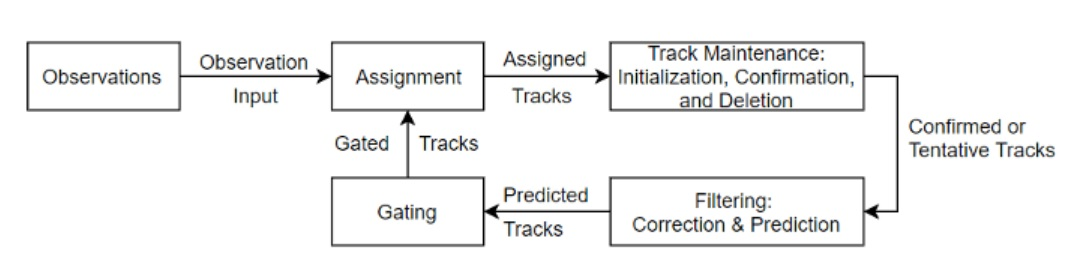
\includegraphics[width=0.9\textwidth]{MTT-figure01.jpg}
\caption{\label{fig:MTT}MTT system.}
\end{figure}

\subsection{MTT system Tables}

Try to use talbes.Just make a table like this.This is Table~\ref{tab:widgets}.

\begin{table}
\centering
\begin{tabular}{l|l|r|r}
Item & X(m) & Y(m) & Z(m) \\\hline
First target & 0 & 0 & 0  \\
second target & 100 & 20 & 10 
\end{tabular}
\caption{\label{tab:widgets}An example of target table.}
\end{table}

\subsection{How to add Comments and Track Changes}

Comments can be added to your project by highlighting some text and clicking ``Add comment'' in the top right of the editor pane\dots

Track changes are available on all our premium plans\dots

\subsection{Try to add Lists of targets}
To interpret this diagram, assume a tracker has maintained confirmed or tentative tracks from the previous scan. Now, the system considers whether to update tracks based on any new detections received from sensors. To assign detections to the corresponding tracks.

\begin{enumerate}
\item The internal filter (such as a Kalman filter) predicts the confirmed or tentative tracks from the previous step to the current step.
\item The tracker uses the predicted estimate and covariance to form a validation gate around the predicted track.
\item The tracker uses the predicted estimate and covariance to form a validation gate around the predicted track.

\begin{itemize}
\item Low-quality tracks are deleted based on the deletion criteria.
\item A tentative track becomes confirmed if the quality of the track satisfies the confirmation criteria.
\end{itemize}
\item The tracker uses the predicted estimate and covariance to form a validation gate around the predicted track.
\end{enumerate}

\subsection{Try to write my Mathematics}

Target distance. First target is $X_1, Y_1,Z_1$,and the second target is $X_2, Y_2,Z_2$ and the distance between first target and the second one $R_1_2$ is:
\[R_1_2 = \sqrt{(X_1-X_2)^2+(Y_1-Y_2)^2+(Z_1-Z_2)^2}\]



\subsection{Try to add a Citations and a References List}
Base on this two method ,Hossein Darvishi proposed a method by using two frequency and complex indicated angles to decrease the multi-path effects. Simulation results show this is a effect way on the monopulse tracking system,and also with low computational complexity and simple implementation\cite{D1} . 


\subsection{Good Try!}

Excellent tools to write a paper,much better than using Office or WPS.

\bibliographystyle{alpha}
\bibliography{sample}

\end{document}
